\documentclass{article}

\usepackage[a4paper, margin=1in]{geometry}
\usepackage{amsmath, amssymb, tikz, centernot}
\usepackage{parskip}
\usepackage[most]{tcolorbox}

\makeatletter
\renewcommand*\env@matrix[1][*\c@MaxMatrixCols c]{%
	\hskip -\arraycolsep
	\let\@ifnextchar\new@ifnextchar
	\array{#1}}
\makeatother

\title{MATH 209: Linear Algebra}
\author{}
\date{}

\begin{document}

\maketitle
\tableofcontents

\break

\section{Vector Space}

A vector space is a non-empty set whose elements are closed under vector addition and scalar multiplication.

\subsection{Axioms}

Suppose $V$ is a non empty set on which two operations are defined: addition of vectors and multiplication by scalars. Then $V$ is a vector space if $\forall \; \underline{u}, \underline{v}, \underline{w} \in V$ and $k,l \in \mathbb{R}$, the following properties hold:
\begin{itemize}
	\item $\underline{u} + \underline{v} \in V$ (closure property under addition)
	\item $\underline{u} + \underline{v} = \underline{v} + \underline{u}$ (commutative property of vector addition)
	\item $\underline{u} + (\underline{v} + \underline{w}) = (\underline{u} + \underline{v}) + \underline{w}$ (associative property of vector addition)
	\item $\exists \; \underline{0} \in V \text{ st } \underline{u} + \underline{0} = \underline{0} + \underline{u} = \underline{u}$ (additive identity)
	\item $\forall \; \underline{u} \in V, \exists \; -u \text{ st } \underline{u} + (-\underline{u}) = -\underline{u} + \underline{u} = \underline{0}$ (additive inverse)
	\item $k\underline{u} \in V$ (closure property under scalar multiplication)
	\item $k(\underline{u} + \underline{v}) = k\underline{u} + k\underline{v}$ (distributive property of scalar multiplication over addition)
	\item $(k+l)\underline{u} = k\underline{u} + l\underline{u}$ (distributive property of scalar multiplication over addition)
	\item $(kl)\underline{u} = k(l\underline{u})$ (associative property of scalar multiplication)
	\item $1\underline{u} = \underline{u}$ (multiplicative identity)
\end{itemize}

Important results derived from these axioms include:
\begin{itemize}
	\item $(-1)\underline{u} = -\underline{u}$
	\begin{tcolorbox}[colback=lightgray!20, colframe=lightgray!20]
		$(-1)\underline{u} = -\underline{u} \iff \underline{u} + (-1)\underline{u} = \underline{0}$. \\
		LHS $= \underline{u} + (-1)\underline{u} = 1\underline{u} + (-1)\underline{u} = (1+(-1))\underline{u} = 0\underline{u} = \underline{0} =$ RHS
	\end{tcolorbox}
	\item $0\underline{u} = \underline{0}$
	\begin{tcolorbox}[colback=lightgray!20, colframe=lightgray!20]
		LHS $= 0\underline{u} = (1+(-1))\underline{u} = 1\underline{u} + (-1\underline{u}) = \underline{u} - \underline{u} = \underline{0} =$ RHS
	\end{tcolorbox}
\end{itemize}

\subsection{Subspace}

$W \subseteq V$ is a subspace if and only if $W$ is itself a vector space, i.e. closed under vector addition and scalar multiplication, i.e.
\begin{itemize}
	\item  $\underline{u} + \underline{v} \in V$ (closure property under addition)
	\item $k\underline{u} \in V$ (closure property under multiplication)
\end{itemize}
\begin{tcolorbox}[colback=lightgray!20, colframe=lightgray!20, fontupper=\linespread{1.25}\selectfont]
	$(\Rightarrow)$ Let $W$ be a subspace of $V$, then all axioms are satisfied including both closures. \\\\	
	$(\Leftarrow)$ Let $W \subseteq V$ be closed under vector addition and scalar multiplication. \\
	Since $W \subseteq V$, all axioms except additive identity and additive inverse hold. \\
	To show that these hold as well, consider the closure property under scalar multiplication, then: \\
	If $k=0 \Rightarrow 0\underline{u} = \underline{0} \in W$ \\
	If $k=-1 \Rightarrow -1\underline{u} = -\underline{u} \in W$	
\end{tcolorbox}

\newpage

\section{Linear Combination}

Let $V = \{\underline{v_i}: i \in I\}$ be a vector space and $S = \{\underline{v_j}: j \in J\} \subseteq V$, where $I = \{1,2,\dots,n\}$ and $J = \{1,2,\dots,r\}$. Then $\underline{v} \in V$ can be expressed as a linear combination of vectors in $S$.

\subsection{Linear Independent}

Consider the additive identity as the linear combination of all vectors in $S$, i.e.
$$\underline{0} = \sum_{j=1}^{r}k_j\underline{v_j}$$
The trivial solution ($k_j = 0$) will always satisfy this expression. If this is the only solution, then $S$ is linearly independent. However if there exists additional non-trivial solution(s), then $S$ is linearly dependent.

If $|S| = 1$, then it is linearly dependent if and only if $\underline{v} = 0$. If $|S| \geq 2$, then it is linearly dependent if and only if any $\underline{v} \in S$ can be expressed as a linear combination of other vectors in $S$.

\subsection{Span}

Consider $\underline{v_i }\in V$ as a linear combination of vectors in $S$, i.e.
$$\underline{v_i} = \sum_{j =1}^{r}k_j\underline{v_j}$$
If all vectors in $V$ can be written as a linear combination of $S$, then $S$ is said to span $V$.

\subsection{Basis}

If $S$ is linearly independent and spans $V$, then $S$ is said to be a basis of $V$ and the cardinality (size) of the basis is the dimension of that space, i.e. $\dim(V) = |S|$.

If $V$ is a $n$-dimensional space and $|S| = n$, then $S$ is a basis if it spans $V$ or is linearly independent.

\section{Linear Systems}

A system of linear equations can be expressed as $A\underline{X} = \underline{B}$ where $A$ is a $m \times n$ coefficient matrix, $\underline{X}$ is a $n\times 1$ variable vector and $\underline{B}$ is a $m \times 1$ solution vector.

$$ A\underline{X} = \underline{B} \hspace{0.5cm} \Rightarrow \hspace{0.5cm}
\begin{bmatrix}
	a_{11} & a_{12} & \dots & a_{1n} \\
	a_{21} & a_{22} & \dots & a_{2n} \\
	\vdots & \vdots & & \vdots \\
	a_{m1} & a_{m2} & \dots & a_{mn} \\
\end{bmatrix}
\begin{bmatrix} x_1 \\ x_2 \\ \vdots \\ x_n \\ \end{bmatrix} =
\begin{bmatrix} b_1 \\ b_2 \\ \vdots \\ b_m \\ \end{bmatrix}
$$

\subsection{Solving a Linear System}

Solving a linear system requires elementary row operations, i.e.
\begin{itemize}
	\item $R_i \rightarrow kR_i$, where $k \not= 0$.
	\item $R_i \leftrightarrow R_j$, where $i \not= j$.
	\item $R_i \rightarrow R_i + kR_j$, where $k \not= 0$ and $i \not= j$.
\end{itemize}

\newpage

To solve a linear system $A\underline{X}=\underline{B}$,
\begin{enumerate}
	\item Construct the augmented matrix, 
	$$ [A|\underline{B}] = \begin{bmatrix}[cccc|c]
		a_{11} & a_{12} & \dots & a_{1n} & b_1 \\
		a_{21} & a_{22} & \dots & a_{2n} & b_2 \\
		\vdots & \vdots &  & \vdots & \vdots \\
		a_{m1} & a_{m2} & \dots & a_{mn} & b_m \\
	\end{bmatrix}$$
	\item Evaluate the Row Echelon Form (Gaussian Elimination) using elementary row operations.
	\begin{itemize}
		\item The first non-zero element in a row must be 1 (known as leading one).
		\item All rows containing only 0 must be grouped at the bottom.
		\item The leading one of each successive row must be to the right of the previous row's leading one.
	\end{itemize}
	\item Evaluate the Reduced Row Echelon Form (Gauss-Jordan Elimination) using elementary row operations.
	\begin{itemize}
		\item The matrix must be in Row Echelon Form.
		\item If a column contains a leading one, all other entries in that column must be 0.
	\end{itemize}
	\item Determine the free (not corresponding to leading ones) and leading variables (corresponding to leading ones), i.e. if $a_{ij}$ is a leading one, then $x_j$ is leading variable.
	\item Rewrite the leading variables in terms of free variables.
	\item Evaluate the reduced system to determine the infinite non-trivial solutions of the form
	$$\underline{X} = \sum_{j = 1}^r t_j \underline{v_j}$$
	where $v_j \in V$ and $t_j$ is some variable.
\end{enumerate}

\subsection{Subspaces of a Homogeneous Linear System}

Consider a homogeneous system ($\underline{B} = \underline{0})$ and let $A$ be a square matrix of order $n$. Then there exists at least the trivial solution, i.e. $\underline{X} = \underline{0}$. If $A$ is invertible ($\exists A^{-1}$ and $\det(A) \not= 0$), then this is the only solution of the system. However, if $A$ is singular ($\centernot{\not\exists} A^{-1}$ and $\det(A) = 0$), then the system has infinite non-trivial solutions as well. 

For a homogeneous system with non-trivial solutions, the following subspaces exist:
\begin{itemize}
	\item Null space of $A$: solution space of $A$,
	$$N(A) = \{\underline{X} \in \mathbb{R}^n: A\underline{X} = \underline{0}\}$$
	\item Row space of $A$: space spanned by the row vectors of $A$,
	$$R(A) = \left\{\underline{u} \in \mathbb{R}^n: \underline{u} = \sum_{i=1}^{m} k_i\underline{r_i}\right\} \text{ where } \underline{r_i} = (a_{i1}, a_{i2}, \dots, a_{in}) \subseteq \mathbb{R}^n$$
	\item Column space of $A$: space spanned by the column vectors of $A$,
	$$C(A) = \left\{\underline{u} \in \mathbb{R}^m: \underline{u} = \sum_{i=1}^{n} k_i\underline{c_i}\right\} \text{ where } \underline{c_i} = (a_{1i}, a_{2i}, \dots, a_{mi}) \subseteq \mathbb{R}^m$$
\end{itemize}

\newpage

\textbf{Dimension Theorem for Matrices}: For a square matrix $A_{n \times n}$, $nullity(A) + rank(A) =  n$, where $nullity = \dim(N)$ or the number of free variables (rows without leading ones) in (reduced) row echelon form of $A$ and $rank(A) = \dim(R) = \dim(C)$. Rank can also be determined by evaluating the
\begin{itemize}
	\item number of linearly independent vectors in $R$ or $C$.
	\item number of non-multiple vectors in $R$ or $C$.
	\item highest order of the non-zero determinant of $A$.
	\item number of leading variables (rows with leading ones) in (reduced) row echelon form of $A$.
\end{itemize}

\subsection{Inferences From Row Echelon Form}

Let $F$ be the (reduced) row echelon form of $A$, then: 
\begin{itemize}
	\item The rows with leading ones form a basis for $R(A)$ and $R(F)$. Because row operations consist of scalar multiplication and vector addition, therefore $F \in R(A) \subseteq \mathbb{R}^n$.
	\item The columns with leading ones form a basis for $C(F)$ but not for $C(A)$. Because row operations change the column space. However, the columns in $A$ corresponding to the columns in $F$ with leading ones form the basis for $C(A)$.
\end{itemize}

Given a homogeneous system, let $S= \{\underline{v_j}: j \in J\}$ be the set of vectors determined from the reduced system. Since the leading variables were written in terms of free variables, $S$ is linearly independent. And since the linear combination of its vectors form a general vector, $S$ spans the solution space as well. Hence $S$ forms the basis for the null space and $\dim(N) = nullity(A) = |S|$.

\section{Inner Product}

\subsection{Euclidean Inner Product}

A vector $\vec{u} = |\vec{u}| \underline{u} = (u_1, u_2, \dots, u_n)$, where $\underline{u}$ is the unit vector (length 1) and the length of a vector is
$$|\vec{u}| = \sqrt{(u_1^2 + u_2^2 + \dots + u_n^2)} = (\vec{u} \cdot \vec{u})^{1/2}$$
Let $\vec{u}, \vec{v} \in \mathbb{R}^n$, then their dot product (aka euclidean inner product) is defined as
$$\vec{u} \cdot \vec{v} = u_1v_1 + u_2v_2 + \dots + u_nv_n = \begin{cases} 0 & \vec{u} = 0 \text{ or } \vec{v} = 0 \\ ||\vec{u}|| \cdot ||\vec{v}||\cos\theta & \vec{u}, \vec{v} \not= 0\end{cases}$$
Moreover, properties of dot product include:
\begin{itemize}
	\item $\vec{u} \cdot \vec{v} = \vec{v} \cdot \vec{u}$
	\item $(\vec{u} + \vec{v}) \cdot \vec{w} = \vec{u} \cdot \vec{w} + \vec{u} \cdot \vec{w}$
	\item $k(\vec{u} \cdot \vec{v}) = (k\vec{u}) \cdot \vec{v} = \vec{u} \cdot (k\vec{v})$
	\item $\vec{u} \cdot \vec{u} \geq 0$ and $\vec{u} \cdot \vec{u} = 0 \iff \vec{u} = \vec{0}$
	\item $\vec{u} \cdot \vec{v} = 0 \iff \vec{u}, \vec{v}$ are perpendicular to one another
\end{itemize}

\phantom{}

All vectors in $\mathbb{R}^n$ have $n$ perpendicular components (projections on $n$ axis). For simplicity, consider $\vec{u} \in \mathbb{R}^2$, then $\vec{u} = \vec{v_1} + \vec{v_2}$ where $\vec{v_1}, \vec{v_2}$ are perpendicular components of $u$ and $\vec{v_1}$ is a scalar vector of $\vec{a}$. Then $\vec{w_1}$ is the projection of $\vec{u}$ along $\vec{a}$, i.e. $$\vec{w_1} = proj_{\underline{a}}\underline{u} = \frac{(\vec{u} \cdot \vec{a}) \vec{a}}{|\vec{a}|^2}$$ and $\vec{w_2}$ (perpendicular to $\vec{a}$) is determined by $\vec{w_2} = \vec{u} - \vec{w_1}$

\begin{tcolorbox}[colback=lightgray!20, colframe=lightgray!20, fontupper=\linespread{1.5}\selectfont]
	\begin{center}
		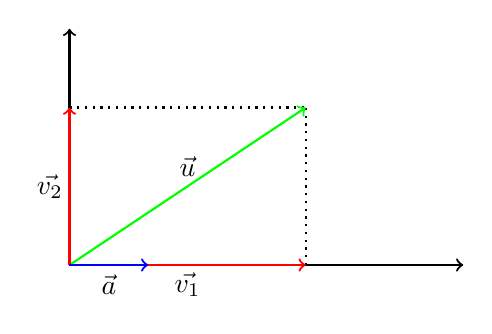
\begin{tikzpicture}
			\draw[thick, ->] (0,0) -- (5,0); % x axis
			\draw[thick, ->] (0,0) -- (0,3); % y axis
			\draw[thick, black, dotted] (0,2) -- (3,2); % v1 parallel
			\draw[thick, black, dotted] (3,0) -- (3,2); % v2 parallel
			\draw[thick, ->, green] (0,0) -- (3,2); % u
			\draw[thick, ->, red] (0,0) -- (3,0); % v1
			\draw[thick, ->, red] (0,0) -- (0,2); % v2
			\draw[thick, ->, blue] (0,0) -- (1,0); % a
			% labels
			\node at (1.5,1.25) {$\vec{u}$};
			\node at (1.5,-0.25) {$\vec{v_1}$};
			\node at (-0.25,1) {$\vec{v_2}$};
			\node at (0.5,-0.25) {$\vec{a}$};
			\end{tikzpicture}
	\end{center}
	Let $\vec{u} = \vec{v_1} + \vec{v_2}$ where $\vec{v_1}$ is along $\vec{a}$ and $\vec{v_2}$ is perpendicular to $\vec{a}$ \\
	It is clear that $\vec{v_2} = \vec{u} - \vec{v_1}$ \\
	Let $\vec{v_1} = k\vec{a}$, where $k \in \mathbb{R}$ \\
	$\Rightarrow \vec{u} = k\vec{a} + \vec{v_2}$ \\
	$\Rightarrow \vec{u} \cdot \vec{a} = k\vec{a} \cdot \vec{a} + \vec{v_2} \cdot \vec{a}$ (dot product with $\vec{a}$) \\
	$\Rightarrow \vec{a} \cdot \vec{u} = k||\vec{a}||^2 + 0 \hspace{0.5cm} \because \vec{v_2} \perp \vec{a} \iff \vec{v_2} \cdot \vec{a} = 0$ and $\vec{a} \cdot \vec{a} = ||\vec{a}||^2$ \\
	$\Rightarrow k = \frac{(\vec{a} \cdot \vec{u})}{||\vec{a}||^2}$ \\
	Substituting $k$ into $\vec{v_1} = k\vec{a}$, we get
	$$\vec{v_1} = \frac{(\vec{a} \cdot \vec{u})}{||\vec{a}||^2}\vec{a}$$
\end{tcolorbox}

\subsection{Inner Product Space}

The dot product is an example of the more generalized concept of inner products. Hence, the notations and terms become generalized as well: $\vec{u} \rightarrow \underline{u}$, length $|\vec{u}| \rightarrow$ norm $||\underline{u}||$, perpendicular $\rightarrow$ orthogonal, dot product $\vec{u} \cdot \vec{v} \rightarrow$ inner product $\left<\underline{u}, \underline{v}\right>$. This is necessary as dot product refers to ordinary vectors in $\mathbb{R}^n$ but inner product refers to generalized vectors which can matrices, polynomials, functions etc.

An inner product space is a real vector space with an inner product $\left<\underline{u}, \underline{v}\right> \in \mathbb{R}$ which satisfies the following axioms $\forall \; \underline{u}, \underline{v} \in V$ and $k \in \mathbb{R}$:
\begin{itemize}
	\item $\left<\underline{u}, \underline{v}\right> = \left<\underline{v}, \underline{u}\right>$ (symmetry)
	\item $\left<\underline{u} + \underline{v}, \underline{w}\right> = \left<\underline{u}, \underline{w}\right> + \left<\underline{u}, \underline{w}\right>$ (additivity)
	\item $\left<k\underline{u}, \underline{v}\right> = k\left<\underline{u}, \underline{v}\right>$ (homogeneity)
	\item $\left<\underline{v}, \underline{v}\right> \geq 0$ and $\left<\underline{v}, \underline{v}\right> = 0 \iff \underline{v} = \underline{0}$ (positivity)
\end{itemize}

Important properties of inner products include
\begin{itemize}
	\item Norm of a vector, $||\underline{u}|| = \left<\underline{u}, \underline{v}\right>^{1/2}$
	\item $\underline{u}, \underline{v}$ are orthogonal vectors if and only if $\left<\underline{u}, \underline{v}\right> = 0$. 
	\begin{itemize}
		\item if $\underline{u}, \underline{v} \in \mathbb{R}^n$, then they are orthogonal if and only if $\underline{u} \cdot \underline{v} = 0$.
		\item if $A \in \mathbb{R}^{n\times n}$ (square matrix),  then it is orthogonal if and only if all row/col vectors contained in it are orthogonal to one another, i.e. $\det(A) = \pm 1$. If, additionally, $A^t = A^{-1}$, then $A$ is properly orthogonal.
	\end{itemize}
	\item Orthonormal vectors are those orthogonal vectors whose norms are 1, i.e. $||\underline{u}|| = ||\underline{v}|| = 1$.
	\item $||\underline{u} + \underline{v}||^2 +||\underline{u} - \underline{v}||^2 = 2||\underline{u}||^2 + 2||\underline{v}||^2$
\end{itemize}

\newpage

\subsection{Gram Schmidt Process}

This is used to transform the basis of a vector space into orthogonal and then a orthonormal basis. 

Let $B = \{\underline{u_i}: i \in I\}$ be a basis for a vector space $V$. Then, $B' = \{\underline{v_i}: i \in I\}$ is the orthogonal basis determined by evaluating the projections of basis vectors, i.e.
$$\underline{v_i} = \underline{u_i} - \sum_{j=1}^{i-1} \frac{\left<\underline{u_i}, \underline{v_j}\right> \underline{v_j}}{||\underline{v_j}||^2}  \hspace{0.5cm} \text{where} \hspace{0.5cm} \underline{v_1} = \underline{u_1}$$
And the orthonormal basis $B''$ is determined by dividing the orthogonal vectors by their norm, i.e.
$$B'' = \left\{ \frac{\underline{v_i}}{||\underline{v_i}||}: i \in I\right\}$$

\begin{tcolorbox}[colback=lightgray!20, colframe=lightgray!20, fontupper=\linespread{1.1}\selectfont]
	Since we are considering generalized vectors and spaces, we prove this completely analytically. \\\\	
	Let $B = \{\underline{u_i}\}$ be a basis for $V$, then we must determine an orthogonal basis $B = \{\underline{v_i}\}$. \\\\
	Let $\underline{v_1} = \underline{u_1}$. \\
	Now $\underline{v_2}$ must be orthogonal to $\underline{v_1}$. A vector can be written as the sum of its orthogonal components, therefore consider $\underline{u_2} = k\underline{v_1} + \underline{v_2}$. Taking inner product with $\underline{v_1}$,
	$$\left<\underline{u_2},\underline{v_1}\right> = k\left<\underline{v_1},\underline{v_1}\right> + \left<\underline{v_2},\underline{v_1}\right>
	\Rightarrow \left<\underline{u_2},\underline{v_1}\right> = k||\underline{v_1}||^2 + 0
	\Rightarrow k =  \frac{\left<\underline{u_2},\underline{v_1}\right>}{||\underline{v_1}||^2}$$
	Hence $\underline{v_2}$ becomes
	$$\underline{v_2} = \underline{u_2} - \frac{\left<\underline{u_2},\underline{v_1}\right> \underline{v_1}}{||\underline{v_1}||^2}$$ \\
	Now $\underline{v_3}$ must be orthogonal to $\underline{v_1}$ and $\underline{v_2}$. Similarly, $\underline{u_3} = k_1\underline{v_1} + k_2\underline{v_2} + \underline{v_3}$. Taking inner product with $\underline{v_1}, \underline{v_2}$ and substituting $k_1, k_2$ respectively into the equation, $\underline{v_3}$ becomes
	$$\underline{v_3} = \underline{u_3} - \frac{\left<\underline{u_3},\underline{v_1}\right> \underline{v_1}}{||\underline{v_1}||^2} - \frac{\left<\underline{u_3},\underline{v_2}\right> \underline{v_2}}{||\underline{v_2}||^2}$$ \\
	Therefore, this is a recursively defined method where $\underline{v_i}$ must be orthogonal to the previous vectors and can be determined by
	$$\underline{v_i} = \underline{u_i} - \sum_{j=1}^{i-1} \frac{\left<\underline{u_i}, \underline{v_j}\right> \underline{v_j}}{||\underline{v_j}||^2}$$ \\
	Hence $B' = \{v_i\}$ is an orthogonal basis for $V$. \\\\
	To determine an orthonormal basis, we simply divide all vectors in $B'$ by their norm. Hence $\forall \; \underline{v_i} \in B'$,
	$$\left|\left| \frac{\underline{v_i}}{||\underline{v_i}||}\right|\right| = \frac{||\underline{v_i}||}{||||\underline{v_i}||||} = \frac{||\underline{v_i}||}{||\underline{v_i}||} = 1$$
	Therefore $B'' = \left\{ \frac{\underline{v_i}}{||\underline{v_i}||}\right\}$ is an orthonormal basis for $V$.
\end{tcolorbox}

If a set $S = \{\underline{v_i}: i \in I\}$ is a set of orthogonal vectors in an inner product space, then $S$ is linearly independent.

\section{Eigen Space}

If $A$ is a square matrix of order $n$, then a non-empty vector $\underline{X} \in \mathbb{R}^n$ is an eigenvector of $A$ if and only if $A\underline{X} = \lambda \underline{X}$ where $\lambda \in \mathbb{R}$ is an eigenvalue. Hence an eigenvector is a vector which when applied to a matrix has the same effect as multiplying the matrix by a scalar (eigenvalue). This effect can be contraction ($\lambda \in [0,1)$), stretching ($\lambda > 1$) or reversal of direction ($\lambda < 0$).

The roots of the \textbf{characteristic equation of a matrix}, $\det(A - \lambda I) = 0$ are the eigenvalues of $A$ and their corresponding eigenvectors are determined by evaluating $(A-I\lambda)\underline{X} = \underline{0}$

\begin{tcolorbox}[colback=lightgray!20, colframe=lightgray!20, fontupper=\linespread{1.2}\selectfont]
	Consider the equation $A\underline{X} = \lambda \underline{X}$ \\
	$\Rightarrow A\underline{X} - \lambda\underline{X} = \lambda\underline{X} - \lambda\underline{X}$ \\
	$\Rightarrow \underline{X}(A - \lambda I) = \underline{0}$ \\
	$\because \underline{X} \not= \underline{0} \therefore (A - \lambda I) = \underline{0}$ \\
	$\Rightarrow \det(A - \lambda I) = 0$
\end{tcolorbox}

Some interesting properties of eigenvalues include:
\begin{itemize}
	\item Let eigenvector $\underline{X}$ corresponds to an eigenvalue $\lambda$ for $A$, then $\underline{X}$ corresponds to $\lambda^n$ for $A^n$.
	\item $\sum \lambda = \text{tr}(A)$ (trace is the sum of main diagonal entries)
	\item $\prod \lambda = \det(A)$
\end{itemize}

\begin{tcolorbox}[colback=lightgray!20, colframe=lightgray!20, fontupper=\linespread{1.5}\selectfont]
	Consider the characteristic equation $\det(A - \lambda I) = 0$ for a matrix of order 2,
	$$\begin{vmatrix} a-\lambda & b \\ c & d-\lambda \\ \end{vmatrix} = 0$$
	$\Rightarrow (a-\lambda)(d-\lambda) - bc = 0$ \\
	$\Rightarrow \lambda^2 - \lambda(a+d) + ad-bc = 0$ \\
	$\Rightarrow \lambda^2 - \lambda tr(A) + \det(A) = 0$ \\
	Recall that for $ax^2+bx+c=0$ with roots $\alpha, \beta$, it holds that $\alpha + \beta = -\frac{b}{a}$ and $\alpha\beta = \frac{c}{a}$. \\
	$\because \lambda_1, \lambda_2$ are roots of the characteristic equation $\therefore \lambda_1 + \lambda_2 = \text{tr}(A)$ and $\lambda_1 \lambda_2 = \det(A)$
\end{tcolorbox}

\textbf{Eigen space} of $A$ corresponding to a $\lambda$ are the vectors $\underline{X}$ that satisfy $A\underline{X} = \lambda\underline{X}$. The non-zero vectors in the space comprise the eigenvectors of $A$. \\
If an eigenvalue is repeated $k$ times and the corresponding eigenspace is $k$-dimensional, then the basis vectors are linearly independent and correspond to the eigenvectors.

\subsection{Diagonalization}

Diagonalization is a process to transform a diagonalizable matrix $A$ into a diagonal matrix $D$ using an invertible matrix $P$, i.e. $D = PAP^{-1}$. The column vectors in $P$ are the eigenvectors of $A$ and their corresponding eigenvalues lie on the main diagonal entries of $D$. Hence $A,D$ are said to be similar to one another.

$A$ is diagonalizable if and only if it has $n$ linearly independent eigenvectors.

\begin{tcolorbox}[colback=lightgray!20, colframe=lightgray!20, fontupper=\linespread{1.3}\selectfont]
	$(\Rightarrow)$ If $A$ is diagonalizable, then it has $n$ linearly independent eigenvectors by definition which form a basis for $\mathbb{R}^n$. \\\\	
	$(\Leftarrow)$ Assume $A$ has $n$ linearly independent eigenvectors $\underline{P_i}$ corresponding to $\lambda_i$. \\
	Let $P = [\underline{P_i}]$ be a matrix, then $AP = [A\underline{P_i}]$ \\
	$\because A\underline{P_i} = \lambda_i A \therefore AP = PD$ where $D$ is a diagonal matrix whose entries are $\lambda$. \\
	$\because P_i$ are linearly independent $\therefore rank(P) = n \Rightarrow \det(P) \not= 0 \Rightarrow P$ is invertible. \\
	Hence $AP = PD \Rightarrow D = P^{-1}AP$.
\end{tcolorbox}

\subsection{Orthogonal Diagonalization}

A square matrix $A$ of order $n$ is orthogonally diagonalizable if there exists an orthogonal matrix $P$ st $P^{-1}AP=P^{t}AP$, i.e. $P^{-1} = P^t$. According to the Spectral theorem for matrices, $A$ is orthogonally diagonalizable if and only if it is symmetric.

To determine such a $P$, determine the orthonormal basis of all eigenspaces individually since eigenvectors from different eigenspaces are orthogonal for a symmetric matrix.

\end{document}